\documentclass[12pt]{article}
\usepackage[paper=letterpaper,margin=1.5cm]{geometry}
\usepackage{amsmath}
\usepackage{amssymb}
\usepackage{amsfonts}
\usepackage{mathtools}
%\usepackage[utf8]{inputenc}
%\usepackage{newtxtext, newtxmath}
\usepackage{lmodern}     % set math font to Latin modern math
\usepackage[T1]{fontenc}
\renewcommand\rmdefault{ptm}
%\usepackage{enumitem}
\usepackage[shortlabels]{enumitem}
\usepackage{titling}
\usepackage{graphicx}
\usepackage[colorlinks=true]{hyperref}
\usepackage{setspace}
\usepackage{subfigure} 
\usepackage{braket}
\usepackage{color}
\usepackage{tabularx}
\usepackage[table]{xcolor}
\usepackage{listings}
\usepackage{mathrsfs}
\usepackage{stackengine}
\usepackage{physics}
\usepackage{afterpage}
\usepackage{pdfpages}
\usepackage[export]{adjustbox}
\usepackage{biblatex}

\setstackEOL{\\}

\definecolor{dkgreen}{rgb}{0,0.6,0}
\definecolor{gray}{rgb}{0.5,0.5,0.5}
\definecolor{mauve}{rgb}{0.58,0,0.82}


\lstset{frame=tb,
  language=Python,
  aboveskip=3mm,
  belowskip=3mm,
  showstringspaces=false,
  columns=flexible,
  basicstyle={\small\ttfamily},
  numbers=none,
  numberstyle=\tiny\color{gray},
  keywordstyle=\color{blue},
  commentstyle=\color{dkgreen},
  stringstyle=\color{mauve},
  breaklines=true,
  breakatwhitespace=true,
  tabsize=3
}
\setlength{\droptitle}{-6em}

\makeatletter
% we use \prefix@<level> only if it is defined
\renewcommand{\@seccntformat}[1]{%
  \ifcsname prefix@#1\endcsname
    \csname prefix@#1\endcsname
  \else
    \csname the#1\endcsname\quad
  \fi}
% define \prefix@section
\newcommand\prefix@section{}
\newcommand{\prefix@subsection}{}
\newcommand{\prefix@subsubsection}{}
\renewcommand{\thesubsection}{\arabic{subsection}}
\makeatother
\DeclareMathOperator*{\argmin}{argmin}
\newcommand{\partbreak}{\begin{center}\rule{17.5cm}{2pt}\end{center}}
\newcommand{\alignbreak}{\begin{center}\rule{15cm}{1pt}\end{center}}
\newcommand{\tightalignbreak}{\vspace{-5mm}\alignbreak\vspace{-5mm}}
\newcommand{\hop}{\vspace{1mm}}
\newcommand{\jump}{\vspace{5mm}}
\newcommand{\R}{\mathbb{R}}
\newcommand{\C}{\mathbb{C}}
\newcommand{\N}{\mathbb{N}}
\newcommand{\G}{\mathbb{G}}
\renewcommand{\S}{\mathbb{S}}
\newcommand{\bt}{\textbf}
\newcommand{\xdot}{\dot{x}}
\renewcommand{\star}{^{*}}
\newcommand{\ydot}{\dot{y}}
\newcommand{\lm}{\mathrm{\lambda}}
\renewcommand{\th}{\theta}
\newcommand{\id}{\mathbb{I}}
\newcommand{\si}{\Sigma}
\newcommand{\Si}{\si}
\newcommand{\inv}{^{-1}}
\newcommand{\T}{^\intercal}
\renewcommand{\tr}{\text{tr}}
\newcommand{\ep}{\varepsilon}
\newcommand{\ph}{\varphi}
%\renewcomand{\norm}[1]{\left\lVert#1\right\rVert}
\definecolor{cit}{rgb}{0.05,0.2,0.45}
\addtolength{\jot}{1em}
\newcommand{\solution}[1]{

\noindent{\color{cit}\textbf{Solution:} #1}}

\newcounter{tmpctr}
\newcommand\fancyRoman[1]{%
  \setcounter{tmpctr}{#1}%
  \setbox0=\hbox{\kern0.3pt\textsf{\Roman{tmpctr}}}%
  \setstackgap{S}{-.9pt}%
  \Shortstack{\rule{\dimexpr\wd0+.1ex}{.9pt}\\\copy0\\
              \rule{\dimexpr\wd0+.1ex}{.9pt}}%
}

\newcommand{\Id}{\fancyRoman{2}}

% Enter the specific assignment number and topic of that assignment below, and replace "Your Name" with your actual name.
\title{STAT 30900: Homework 3}
\author{Caleb Derrickson}
\date{November 11, 2023}

\begin{document}
\onehalfspacing
\maketitle
\allowdisplaybreaks
{\color{cit}\vspace{2mm}\noindent\textbf{Collaborators:}} The TA's of the class, as well as Kevin Hefner, and Alexander Cram.

\tableofcontents

\newpage
\section{Problem 1}
Given a symmetric $A \in \R^{n\times n}, \textbf{0} \neq \textbf{x} \in \R^n$, and $\textbf{b} \in \R^n$. Let 
\[
\textbf{r} = \textbf{b} - A\textbf{x}
\]
Consider the $QR$ decomposition
\[
[\textbf{x}, \textbf{r}] = QR
\]
and observe that if $E\textbf{x} = \textbf{r}$, then
\[
(Q^TEQ)(Q^T\textbf{x}) = Q^T\textbf{r}.
\]
Show how to compute a symmetric $E \in \R^{n\times n}$ so that is attains 
\[
\min_{(A+E)\textbf{x} = \textbf{b}}\norm{E}_F
\]
where the minimum is taken over all symmetric $E$.
\partbreak
\begin{solution}

    We are given $[\textbf{x}, \textbf{r}] = QR$, which when multiplied on the left by $Q^T$ implies $[Q^T\textbf{x}, Q^T\textbf{r}] = Q^TQR = R$. Note that $R$ is upper triangular, so $Q^T\textbf{x}$ and $ Q^T\textbf{r}$ will have one and at most two nonzero elements, respectively. We are given the relation between them in the form $ (Q^TEQ)(Q^T\textbf{x}) = Q^T\textbf{r}$ if $E\textbf{x} = \textbf{r}$. Then, we can break this into cases based on the number of elements in $Q^T\textbf{r}$.

    \begin{enumerate}
        \item \underline{Case 1:} $Q^T\textbf{r}$ has one nonzero element. 

        Denote $\Gamma = Q^TEQ$. Then by the relation given, 
        \[
        \Gamma (Q^T\textbf{x}) = \mqty[\cdot &\cdots &\cdot\\ \vdots &\ddots &\vdots\\ \cdot &\cdots &\cdot]\mqty[\vert \\ Q^T\textbf{x} \\ \vert] = \mqty[\alpha \\ \vdots\\0] = \mqty [\Gamma_{11}(Q^T\textbf{x})_1 + \Gamma_{12}(Q^T\textbf{x})_2 + ...\\ \Gamma_{21}(Q^T\textbf{x})_1 + \Gamma_{22}(Q^T\textbf{x})_2 + ...\\ \vdots]
        \]
        Note that the only nonzero element in $Q^T\textbf{r}$ is the first element, so $\Gamma_{j1}(Q^T\textbf{x})_1 + \Gamma_{j2}(Q^T\textbf{x})_2 + ...$ = 0 for $j \neq 1$. The only nonzero element in  $Q^Tx$ is the first, so any terms not involving $Q^T\textbf{x})_1$ is zero. so $\Gamma_{j1}, \Gamma_{j2}, ..., \Gamma_{jn}$ are arbitrary for $j\neq 1$. Since $\gamma$ is symmetric, then $\Gamma_{12}, \Gamma_{13},  ...,\Gamma_{1n}$ are also arbitrary. Then the only non-arbitrary element in $\Gamma$ is $\Gamma_{11}$. Thus, $\min \norm{E}_F = \min \norm{Q^TEQ}_F = \abs{\Gamma_{11}}$ (since all other elements are arbitrary, the minimum is attained when they are 0). Note the second equality holds since the Frobenius norm is unitary invariant. 

\newpage
        \item \underline{Case 2:} $Q^T\textbf{r}$ has two nonzero elements.

        By the same logic in the previous case, 
        \[
        \Gamma (Q^T\textbf{x}) = \mqty[\cdot &\cdots &\cdot\\ \vdots &\ddots &\vdots\\ \cdot &\cdots &\cdot]\mqty[\vert \\ Q^T\textbf{x} \\ \vert] = \mqty[\alpha \\ \beta\\\vdots\\0] = \mqty [\Gamma_{11}(Q^T\textbf{x})_1 + \Gamma_{12}(Q^T\textbf{x})_2 + ...\\ \Gamma_{21}(Q^T\textbf{x})_1 + \Gamma_{22}(Q^T\textbf{x})_2 + ...\\ \vdots]
        \]
        Then the only possible non arbitrary terms are $\Gamma_{11}(Q^T\textbf{x})_1, \Gamma_{12}(Q^T\textbf{x})_2, \Gamma_{21}(Q^T\textbf{x})_1, \Gamma_{22}(Q^T\textbf{x})_2$ by the same logic in the previous case. Note that $(Q^T\textbf{x})_j = 0$ for $j \neq 1$. Then, $\Gamma_{22}(Q^T\textbf{x})_2$ equals 0 for any value of $\Gamma_{22}$, making it arbitrary. Note that $(Q^T\textbf{r})_2$ is nonzero, so this must mean $\Gamma_{21}(Q^T\textbf{x})_1 \neq 0$, meaning $\Gamma_{21} \neq 0$. Since $\Gamma$ is symmetric, this means $\Gamma_{12} \neq 0$. Thus the only non arbitrary elements of $\Gamma$ are $\Gamma_{11}, \Gamma_{12}, \Gamma_{21}$. Therefore, $\min \norm{E}_F^2 = \min \norm{Q^TEQ}_F = |\Gamma_{11}| + |\Gamma_{12}| + |\Gamma_{21}|$.   
        
    \end{enumerate}
\end{solution}


\newpage
\section{Problem 2}
Let $A \in \R^{m \times n}$ and suppose the complete orthogonal decomposition is given by
\[
A = Q_1 \begin{bmatrix}L &0\\0&0\end{bmatrix}Q_2^T
\]
where $Q_1$ and $Q_2$ are orthogonal, and $L$ is a nonsingular lower triangular matrix. Recall that $X \in \R^{n \times m}$ is the unique pseudo-inverse of $A$ is the following Moore-Penrose conditions hold:
\begin{enumerate}[(i)]
    \item $AXA = A$ 
    \item $XAX = X$ 
    \item $(AX)^T = AX$ 
    \item $(XA)^T = XA$
\end{enumerate}
and in which case we write $A^\dag = X$.
\subsection{Problem 2, part a}
Let 
\[
A^- = Q_2\begin{bmatrix}L^\inv &Y \\ 0 &0\end{bmatrix}Q_1^T, \hspace{5mm} Y\neq 0. 
\]
Which of the four conditions (i) - (iv) are satisfied?
\partbreak
\begin{solution}

    We will go straight into calculations.
    \alignbreak
    \begin{align}
        i) \ AXA &=  Q_1 \begin{bmatrix}L &0\\0&0\end{bmatrix}Q_2^T Q_2\begin{bmatrix}L^\inv &Y \\ 0 &0\end{bmatrix}Q_1^T Q_1 \begin{bmatrix}L &0\\0&0\end{bmatrix}Q_2^T &\text{(Given.)}\nonumber\\
        &= Q_1 \begin{bmatrix}L &0\\0&0\end{bmatrix}\begin{bmatrix}L^\inv &Y \\ 0 &0\end{bmatrix}\begin{bmatrix}L &0\\0&0\end{bmatrix}Q_2^T &\text{($Q_1, Q_2$ are orthogonal.)}\nonumber\\
        &=  Q_1 \begin{bmatrix}\id &LY\\0&0\end{bmatrix}\begin{bmatrix}L &0 \\ 0 &0\end{bmatrix}Q_2^T &\text{(Matrix Multiplication.)}\nonumber\\
        &=  Q_1 \begin{bmatrix}L &0 \\ 0 &0\end{bmatrix}Q_2^T &\text{(Matrix Multiplication.)}\nonumber\\
        &= A &\text{(By Definition.)}\nonumber\\
        ii) \ XAX &= Q_2\begin{bmatrix}L^\inv &Y \\ 0 &0\end{bmatrix}Q_1^T Q_1 \begin{bmatrix}L &0\\0&0\end{bmatrix}Q_2^T Q_2\begin{bmatrix}L^\inv &Y \\ 0 &0\end{bmatrix}Q_1^T &\text{(Given.)}\nonumber\\
        &= Q_2\begin{bmatrix}L^\inv &Y \\ 0 &0\end{bmatrix} \begin{bmatrix}L &0\\0&0\end{bmatrix}\begin{bmatrix}L^\inv &Y \\ 0 &0\end{bmatrix}Q_1^T &\text{($Q_1, Q_2$ are orthogonal.)}\nonumber\\
        &= Q_2\begin{bmatrix}\id &0\\0 &0\end{bmatrix}\begin{bmatrix}L^\inv &Y \\0 &0\end{bmatrix}Q_1^T &\text{(Matrix Multiplication.)}\nonumber\\
        &= Q_2\begin{bmatrix}L^\inv &Y \\0 &0\end{bmatrix}Q_1^T&\text{(Matrix Multiplication.)}\nonumber\\
        &= X &\text{(By Definition.)}\nonumber\\
        iii) \ (AX)^T &= \Bigg(Q_1 \begin{bmatrix}L &0\\0&0\end{bmatrix}Q_2^T Q_2\begin{bmatrix}L^\inv &Y \\ 0 &0\end{bmatrix}Q_1^T \Bigg)^T &\text{(Given.)}\nonumber\\
        &= \Bigg(Q_1 \begin{bmatrix}L &0\\0&0\end{bmatrix}\begin{bmatrix}L^\inv &Y \\ 0 &0\end{bmatrix}Q_1^T \Bigg)^T &\text{($Q_2$ is orthogonal.)}\nonumber\\
        &= \Bigg( Q_1\begin{bmatrix}\id &LY \\ 0 &0\end{bmatrix}Q_1^T\Bigg)^T &\text{(Matrix multiplication.)}\nonumber\\
        &=  Q_1\begin{bmatrix}\id &0 \\ LY &0\end{bmatrix}Q_1^T &\text{(Transposition.)}\nonumber\\
        &\neq AX &\text{(As can be seen.)}\nonumber\\
        iv) \ (XA)^T &= \Bigg( Q_2 \begin{bmatrix}L^\inv &Y \\ 0&0\end{bmatrix}Q_1^TQ_1\begin{bmatrix}L &0\\0 &0\end{bmatrix}Q_2^T\Bigg)^T &\text{(Given.)}\nonumber\\
        &= \Bigg( Q_2 \begin{bmatrix}L^\inv &Y \\ 0&0\end{bmatrix}\begin{bmatrix}L &0\\0 &0\end{bmatrix}Q_2^T\Bigg)^T &\text{($Q_1$ is orthogonal.)}\nonumber\\
        &= \Bigg( Q_2 \begin{bmatrix}\id &0 \\ 0 &0\end{bmatrix}Q_2^T\Bigg)^T &\text{(Matrix Multiplication.)}\nonumber\\
        &= Q_2 \begin{bmatrix}\id &0 \\ 0 &0\end{bmatrix}Q_2^T &\text{(Transposition.)}\nonumber\\
        &= XA &\text{(As can be seen.)}\nonumber
    \end{align}
    \alignbreak
    Thus, we see that $(i), (ii),$ and $(iv)$ hold, but not $(iii)$.
\end{solution}

\newpage
\subsection{Problem 2, part b}
Prove that 
\[
A^\dag = Q_2 \begin{bmatrix}L^\inv &0 \\ 0 &0\end{bmatrix}Q_1^T
\]
by letting 
\[
A^\dag = Q_2\begin{bmatrix}X_{11} &X_{12} \\ X_{21} &X_{22}\end{bmatrix}Q_1^T
\]
and by completing the following steps
\begin{itemize}
    \item Using $(i)$, prove that $X_{11} = L^\inv$.
    \item Using the symmetry conditions $(iii)$ and $(iv)$, prove that $X_{12} = X_{21} = 0$. 
    \item Using $(ii)$, prove that $X_{22} = 0$.
\end{itemize}
\partbreak
\begin{solution}

    Here we are letting the middle term take on any form (within reason), then arguing by the properties of the Moore-Penrose pseudo-inverse, that it must take this form. Then, let 
    \[
    A^\dag = Q_2\begin{bmatrix}X_{11} &X_{12} \\ X_{21} &X_{22}\end{bmatrix}Q_1^T
    \]

    We will then recover terms by the above properties in the suggested order.
    \begin{itemize}
        \item By the first property, $AXA = A$ must be obeyed. Then, 
        \vspace{-5mm}
        \alignbreak
        \vspace{-5mm}
        \begin{align}
            AA^\dag A &= Q_1\begin{bmatrix}L &0\\0&0\end{bmatrix}Q_2^TQ_2\begin{bmatrix}X_{11} &x_{12}\\X_{21} &X_{22}\end{bmatrix}Q_1^TQ_1\begin{bmatrix}L &0\\0&0\end{bmatrix} &\text{(Given.)}\nonumber\\
            &=  Q_1\begin{bmatrix}L &0\\0&0\end{bmatrix}\begin{bmatrix}X_{11} &x_{12}\\X_{21} &X_{22}\end{bmatrix}\begin{bmatrix}L &0\\0&0\end{bmatrix} &\text{($Q_1, Q_2$ are orthogonal.)}\nonumber\\
            &= Q_1 \begin{bmatrix}LX_{11} &LX_{12}\\ 0&0\end{bmatrix}\begin{bmatrix}L &0\\0&0\end{bmatrix}Q_2^T &\text{(Matrix multiplication.)}\nonumber\\
            &= Q_1\begin{bmatrix}LX_{11}L &0 \\0&0\end{bmatrix}Q_2^T &\text{(Matrix multiplication.)}\nonumber\\
            \implies &LX_{11}L = L &(AA^\dag A = A.)\nonumber\\
            \iff &X_{11} = L^\inv &\text{($L$ is nonsingular.)}\nonumber
        \end{align}
        \alignbreak
        \vspace{-5mm}
        \newpage
        \item Next, we will take the symmetric properties of the Moore-Penrose pseudo inverse.
        \alignbreak
        \begin{align}
        AA^\dag &= \Bigg( Q_1\begin{bmatrix}L &0\\0 &0\end{bmatrix}Q_2^TQ_2\begin{bmatrix}L^\inv &X_{12}\\ X_{21} &X_{22}\end{bmatrix}Q_1^T\Bigg)^T &\text{(Given.)}\nonumber\\
        &= \Bigg( Q_1\begin{bmatrix}L &0\\0 &0\end{bmatrix}\begin{bmatrix}L^\inv &X_{12}\\ X_{21} &X_{22}\end{bmatrix}Q_1^T\Bigg)^T &\text{($Q_2$ is orthogonal.)}\nonumber\\
        &= \Bigg( Q_1\begin{bmatrix}\id &LX_{12}\\0 &0\end{bmatrix}Q_1^T\Bigg)^T &\text{(Matrix multiplication.)}\nonumber\\
        \implies LX_{12} &= L &\text{(Transposition and $(AA^\dag)^T = AA^\dag$.)}\nonumber\\
        \implies \ \  X_{12} &= 0 &\text{($L$ is nonsingular, thus nonzero.)}\nonumber\\
        (A^\dag A)^T &= \Bigg( Q_2 \begin{bmatrix}L^\inv &0 \\X_{21} &X_{22}\end{bmatrix}Q_1^TQ_1\begin{bmatrix}L &0\\0&0\end{bmatrix}Q_2^T\Bigg)^T &\text{(Given.)}\nonumber\\
        &= \Bigg( Q_2 \begin{bmatrix}L^\inv &0 \\X_{21} &X_{22}\end{bmatrix}\begin{bmatrix}L &0\\0&0\end{bmatrix}Q_2^T\Bigg)^T &\text{($Q_1$ is orthogonal.)}\nonumber\\
        &= \Bigg( Q_2 \begin{bmatrix}\id &0 \\X_{21}L &0\end{bmatrix}Q_2^T\Bigg)^T &\text{(Matrix multiplication.)}\nonumber\\
        \implies X_{21}L &= 0 &\text{(Transposition and $(A^\dag A)^T = A^\dag A$.)}\nonumber\\
        \implies \ \ X_{21} &= 0 &\text{(L is invertible thus nonzero.)}\nonumber
        \end{align}
        \alignbreak
        
        \item Finally, we will show $X_{22} = 0$.
        \alignbreak
        \begin{align}
            A^\dag AA^\dag &= Q_2\begin{bmatrix}L^\inv &0 \\ 0 &X_{22}\end{bmatrix}Q_1^TQ_1 \begin{bmatrix}L &0\\ 0 &0\end{bmatrix}Q_2^TQ_2 \begin{bmatrix}L^\inv &0 \\0 &X_{22}\end{bmatrix}Q_1^T &\text{(Given.)}\nonumber\\
            &= Q_2\begin{bmatrix}L^\inv &0 \\ 0 &X_{22}\end{bmatrix} \begin{bmatrix}L &0\\ 0&0\end{bmatrix} \begin{bmatrix}L^\inv &0 \\0 &X_{22}\end{bmatrix}Q_1^T &\text{($Q_1, Q_2$ are orthogonal.)}\nonumber\\
            &= Q_2\begin{bmatrix}\id &0\\0&0\end{bmatrix}\begin{bmatrix}L^\inv &0 \\ 0&X_{22}\end{bmatrix}Q_1^T &\text{(Matrix multiplication.)}\nonumber\\
            &= Q_2\begin{bmatrix}L^\inv &0 \\0&0\end{bmatrix}Q_1^T &\text{(Matrix multiplication.)}\nonumber\\
            \implies X_{22} &= 0 &(A^\dag AA^\dag = A^\dag.) \nonumber
        \end{align}
        \alignbreak
    \end{itemize}

    Therefore, $A^\dag$ is of the given form. Note that I passed over some steps, including steps where I equated entries only in the block matrix, ignoring the factors which would appear when multiplied by $Q_i$ for its transpose. Since they are orthonormal however, these factors will cancel out, leaving us only with the entry in the block matrix. 
\end{solution}

\newpage
\section{Problem 3}
Let $A \in \R^{m \times n}, \textbf{b} \in \R^m,$ and $\textbf{c}\in \R^n$. We are interested in the least squares problem
\begin{align}
    \min_{\textbf{x}\in \R^n} \norm{A\textbf{x} - \textbf{b}}^2_2 \label{p3: min}
\end{align}
\subsection{Problem 3, part a}
Show that \textbf{x} is a solution to (\ref{p3: min}) if and only if \textbf{x} is a solution to the \textit{augmented system}
\begin{align}
    \begin{bmatrix}\id &A\\A^T&0\end{bmatrix}\begin{bmatrix}\textbf{r}\\\textbf{x}\end{bmatrix} = \begin{bmatrix}\textbf{b}\\0\end{bmatrix} \label{p3: augmented soln}
\end{align}
\partbreak
\begin{solution}

    \begin{itemize}
        \item $\underline{\implies}):$ Suppose (\ref{p3: min}) $\implies$ (\ref{p3: augmented soln}) were false, that is, $\textbf{x}$ is not a solution to the augmented system. Note that since $\textbf{x}$ is a solution to (\ref{p3: min}), then $A\textbf{x} - \textbf{b} = \textbf{d}$, for some $\textbf{d}$. Note that $\textbf{d}$ is in general nonzero. For simplicity, we will break this proof down into cases. 

        \begin{itemize}
            \item \underline{Case 1:} $\textbf{b} \in$ im $(A)$.

            Then the minimum of $\norm{A\textbf{x} - \textbf{b}}$ would equal zero, since $\norm{A\textbf{x - \textbf{b}}} = \norm{A(\textbf{x} - \textbf{y})} = 0$, which attains minimum when $\textbf{x} = \textbf{y}$, meaning $A\textbf{x} = \textbf{b}$. Then $\textbf{d} = 0$. Then (\ref{p3: augmented soln}) simplifies to
            \[
            \begin{bmatrix}\id &A\\ A^T& 0\end{bmatrix}\begin{bmatrix}\textbf{0}\\ \textbf{x}\end{bmatrix} = \begin{bmatrix}\textbf{b}\\0\end{bmatrix}.
            \]
            This implies $A\textbf{x} = b$ and $A^T\textbf{0} = \textbf{0}$. Since these are both true, then we run into a contradiction.
            \item \underline{Case 2:} $\textbf{b} \notin$ im $(A)$

            Then $\norm{A\textbf{x} - b} \neq 0$. This would mean $\textbf{d} \neq 0$, and $\textbf{d} \neq $ im$(A)$ since if it were, then we can write $\textbf{d} = A\textbf{y}$, then $\norm{A(\textbf{x} - \textbf{y}) - b} = 0$, which means $\textbf{x} - \textbf{y}$ is a solution to (\ref{p3: min}), meaning $\textbf{x}$ is not a minimum, which is a contradiction. Since $\textbf{d} \notin$ im $(A)$, then $\textbf{d} \in \ker (A^T)$ by the Fredholm Alternative. Then (\ref{p3: augmented soln}) is equivalent to
            \[
            \begin{bmatrix}\id &A\\ A^T& 0\end{bmatrix}\begin{bmatrix}\textbf{d}\\ \textbf{x}\end{bmatrix} = \begin{bmatrix}\textbf{b}\\0\end{bmatrix}.
            \]
            This implies $A\textbf{x} + \textbf{d} = \textbf{b}$ and $A^T\textbf{d} = 0$. This is is true, since we only know $\textbf{d}$ up to sign. Thus (\ref{p3: augmented soln}) holds, giving us a contradiction. 
        \end{itemize}

        \item $\underline{\impliedby}):$

        Note that (\ref{p3: augmented soln}) is equivalent to $A\textbf{x} + \textbf{b} = \textbf{r}$ and $A^T\textbf{r} = 0$. We will again break this down into cases. 

        \begin{itemize}
            \item \underline{Case 1:} $\textbf{b} \in $ im$(A)$. 

            Then $\textbf{b} = A\textbf{y}$ for some $\textbf{y} \in \R^n$. Thus $\textbf{r}= A\textbf{x} + \textbf{b} = A(\textbf{x} - \textbf{y})$. Thus when taking the minimum over all $\textbf{x}$, we see that $\norm{A(\textbf{x} - \textbf{y})} = 0$, exactly when $\textbf{x} = \textbf{y}$. Since $\norm{\cdot}_2$ is positive, then $\textbf{x} \in \argmin (\norm{A\textbf{x} - \textbf{b}})$, which means $\textbf{x}$ is a solution to (\ref{p3: min}).

            \item \underline{Case 2:} $\textbf{b}\notin$ im$(A)$.

            Then, by the Fredholm Alternative, $\textbf{b} \in \ker(A^T)$. Thus, the following can be shown:
            \alignbreak
            \begin{align}
                \norm{\textbf{r}}_2^2 &= \norm{A\textbf{x} - \textbf{b}}_2^2 = (A\textbf{x} - \textbf{b})^T(A\textbf{x} - \textbf{b}) &\text{(2-norm, given.)}\nonumber\\
                &= \textbf{x}^TA^TA\textbf{x} - \textbf{x}^TA^T\textbf{b} - \textbf{b}^TA\textbf{x} + \textbf{b}^T\textbf{b} &\text{(Factoring out.)}\nonumber\\
                &= \textbf{x}^TA^TA\textbf{x}  - \textbf{b}^TA\textbf{x} + \textbf{b}^T\textbf{b} &(\textbf{b} \in \ker(A^T).)\nonumber\\
                &= \textbf{x}^TA^TA\textbf{x}  - (A^T\textbf{b})^T\textbf{x} + \textbf{b}^T\textbf{b} &\text{(Associativity.)}\nonumber\\
                &= \textbf{x}^TA^TA\textbf{x} + \textbf{b}^T\textbf{b} &(\textbf{b} \in \ker(A^T).)\nonumber\\
                &= \norm{A\textbf{x}}_2^2 + \norm{\textbf{b}}_2^2 &\text{(2-norm definition.)}\nonumber
            \end{align}
            \alignbreak

            This then means that $\textbf{x}$ satisfies the Pythagorean Theorem, implying that $\textbf{x}$ is a solution to (\ref{p3: min}). 
        \end{itemize}
    \end{itemize}
\end{solution}

\newpage
\subsection{Problem 3, part b}
Show that the $(m + n) \times (m + n)$ matrix in (\ref{p3: augmented soln}) is nonsingular if and only if $A$ has full column rank.
\partbreak
\begin{solution}

    Denote $\A$ to be the $(m + n) \times (m + n)$ matrix in (\ref{p3: augmented soln}). We will again break this down into cases. 

    \begin{itemize}
        \item $\underline{\implies}):$ 

        Suppose false, that is, $\A$ is singular, but $A$ has full column rank. Note this means $A$ has full rank. Since $\A$ is singular, then $\exists \textbf{v} \in \R^{m + n} \setminus \{\textbf{0}\}$ which is mapped to $\textbf{0}$ under $\A$. Let $\textbf{v} = [\textbf{v}_\textbf{r}, \textbf{v}_\textbf{x}]^T$. This then means, by (\ref{p3: augmented soln}), that  $\textbf{v}_\textbf{r} + A\textbf{v}_\textbf{x} = 0$ and $A^T\textbf{v}_\textbf{r} = 0$. We can substitute the first equation into the second to get $A^TA\textbf{v}_\textbf{x} = 0$. Note that if $A$ is full rank, then $A^T$ is also full rank. This means that $A\textbf{v}_\textbf{x} \in \ker(A^T)$. Since $A^T$ has full rank, this means $\textbf{v}_\textbf{x} \in \ker(A)$, which means $\textbf{v}_\textbf{x} =0 $, since $A$ is full rank. Then, since $A\textbf{v}_\textbf{x} = -\textbf{v}_\textbf{r}, \implies \textbf{v}_\textbf{r} = 0$ as a result. Note we assumed that $\textbf{v} \neq 0$, which is a contradiction, since $\textbf{v}$ was found to only be zero. 

        \item $\underline{\impliedby}):$

        This is equivalent to showing $\det (\A) \neq 0$. Note that in general, a $2\times 2$ block matrix has determinant
        \[
        \det \Bigg( \begin{bmatrix}A &B\\C &D\end{bmatrix}\Bigg) = \det(A)\det(D - CA^\inv B)
        \]

        With $\A$, this then means $\det(\A) = \det(\id)\det(0 - A^T(\id)^\inv A) = det(-A^TA) = (-1)^n\det(A^TA)$. Note that $A^TA$ has full rank when $A$ has full rank. Furthermore, $A^TA$ is normal, thus its SVD decomposition coincides with an eigenvalue decomposition, with $\sigma^2 = \lm$. since $A$ has full rank, then all singular values of $A^TA$ are nonzero, thus all eigenvalues are nonzero, thus $\det(A^TA) \neq 0$. Therefore $\det(\A) \neq 0$ when $A$ has full column rank. 
    \end{itemize}
\end{solution}

\newpage
\subsection{Problem 3, part c}
Suppose $A$ has full column rank and the $QR$ decomposition of $A$ is 
\[
A = Q\begin{bmatrix}R\\0\end{bmatrix}.
\]
Show that he solution to the augmented system
\[
\begin{bmatrix}\id &A\\A^T &0\end{bmatrix}\begin{bmatrix}\textbf{y}\\\textbf{x}\end{bmatrix}
=
\begin{bmatrix}\textbf{b}\\\textbf{c}\end{bmatrix}
\]
can be computed from
\[
\textbf{x} = (R^\inv)^T \textbf{c}, \hspace{5mm} \begin{bmatrix}\textbf{d}_1\\\textbf{d}_2\end{bmatrix} = Q^T\textbf{b},
\]

and
\[
\textbf{x} = R^\inv(\textbf{d}_1 - \textbf{z}), \hspace{5mm }\textbf{y} = Q\begin{bmatrix}\textbf{z}\\\textbf{d}_2\end{bmatrix}.
\]
\partbreak
\begin{solution}

    This is just an exercise in reverse engineering, and computation. We can recover the first equation in the following steps:

    \alignbreak
    \begin{align*}
        Q^T\textbf{b} &= \mqty[\textbf{d}_1\\\textbf{d}_2] &\text{(Given.)}\\
        &= \mqty[\textbf{d}_1 + \textbf{z} - \textbf{z}\\\textbf{d}_1] &\text{(Adding a zero.)}\\
        &= \mqty[\textbf{z}\\\textbf{d}_2] + \mqty[\textbf{d}_1 - \textbf{z}] &\text{(Separating.)}\\
        &= \mqty[\textbf{z}\\\textbf{d}_2] + \mqty[R\\0] R^\inv(\textbf{d}_1 - \textbf{z}) &(R^\inv R = \id.)\\
        &= Q^T\Bigg(Q\mqty[\textbf{z}\\\textbf{d}_2]\Bigg) + \mqty[R\\0] R^\inv(\textbf{d}_1 - \textbf{z}) &(Q^TQ = \id.)\\
        \implies Q^T\textbf{b} &= Q^T\textbf{y} + \mqty[R\\0]\textbf{x} &\text{(Given definitions.)}\\
        \implies \textbf{b} &= \textbf{y} + Q\mqty[R\\0] \textbf{x} &\text{(Multiplying by $Q$.)}\\
        \implies \textbf{b} &= \textbf{y} + A\textbf{x} &\text{($QR$ of $A$.)}
    \end{align*}
    \alignbreak

    The second equation can also be found similarly. 
    \alignbreak
    \begin{align*}
        \textbf{z} &= (R^\inv)^T\textbf{c} &\text{(Given.)}\\
        \implies \ \ \textbf{z}^T &= \textbf{c}^TR^\inv &\text{(Transposition.)}\\
        \implies \ \ \textbf{c}^T &= \textbf{z}^TR &\text{(Multiplying by $R$.)}\\
        \implies  \textbf{c} &= R^T\textbf{z} &\text{(Transposition.)}\\
        &= \mqty[R^T&0] \mqty[\textbf{z}\\\textbf{d}_2] &\text{(Block Equivalence, element of $\textbf{d}_2$ could be anything.)}\\
        &= \mqty[R^T&0] Q^TQ\mqty[\textbf{z}\\\textbf{d}_2] &(Q^TQ = \id.)\\
        &= \Bigg( Q\mqty[R\\0]\Bigg)^TQ\mqty[\textbf{z}\\\textbf{d}_2] &\text{(Transposition.)}\\
        \implies \textbf{y} &= A^T\textbf{y} &\text{(Given definitions.)}
    \end{align*}
    \alignbreak
\end{solution}

\newpage
\subsection{Problem 3, part d}
Hence deduce that if $A$ has full column rank, then 
\[
A^\dag = R^\inv Q^T_1
\]
where $Q = [Q_1, Q_2]$ with $Q_1 \in \R^{m\times n}$ and $Q_2 \in \R^{m\times (m - n)}$. Check this agrees with the general formula derived for a rank-retaining factorization $A = GH$ in the lectures. 

\partbreak
\begin{solution}

    We first show that the given $A^\dag$ satisfies the properties of the Moore-Penrose pseudo-inverse:

    \alignbreak
    \begin{align*}
        i) \ AA^\dag A &= (Q\mqty[R\\0]R^\inv Q_1^T)A &\text{(Given.)}\\
        &= \mqty[Q_1\\Q_2] \mqty[R\\0]R^\inv Q_1^T)A &\text{(Definitions.)}\\
        &=  Q_1RR^\inv Q_1^T A &\text{(Matrix multiplication.)}\\
        &= (Q_1Q_1^T)A &\text{($R^\inv R = \id$.)}\\
        &= (Q_1Q_1^T)\mqty[Q_1&Q_2]\mqty[R\\0] &\text{(Writing out.)}\\
        &= Q_1Q_1^TQ_1R &\text{(Matrix Multiplication.)}\\
        &= Q_1R &\text{($Q_1$ has orthonormal columns.)}\\
        ii) \ A^\dag A A^\dag &= R^\inv Q_1^T\mqty[Q_1\\Q_2]\mqty[R\\0]A^\dag &\text{(Given.)}\\
        &= R^\inv Q_1^TQ_1R A^\dag &\text{(Matrix multiplication.)}\\
        &= (\id)A^\dag &\text{($Q_1$ has orthonormal columns, $R^\inv R = \id$.)}\\
        iii) \ (A^\dag A)^T &= \Bigg( R^\inv Q_1^T \mqty[Q_1 &Q_2]\mqty[R\\0]\Bigg)^T &\text{(By definition.)}\\
        &= (R^\inv Q_1^TQ_1R)^T &\text{(Matrix multiplication.)}\\
        &= (R^\inv R)^T &\text{($Q_1$ has orthonormal columns.)}\\
        &= \id &\text{($R^\inv R = \id$)}\\
        iv) \ (AA^\dag)^T &=\Bigg(\mqty[Q_1 &Q_2]\mqty[R\\0]R^\inv Q_1^T\Bigg)^T &\text{(Given.)}\\
        &= \Bigg(Q_1RR^\inv Q_1^T\Bigg)^T &\text{(Matrix multiplication.)}\\
        &= \Bigg(Q_1 Q_1^T\Bigg)^T  &(R^\inv R = \id.)\\
    \end{align*}
    \alignbreak

    Note that I have to be careful in handling the $Q$ subspaces. Since $Q$ had orthonormal columns, $Q_1^T Q_1 = \id$, but $Q_1Q_1^T \neq \id$ in general. However, $(Q_1Q_1^T)^T = Q_1Q_1^T$, Thus $(iv)$ will hold. This issue also pops ups in $(i)$, but problems subside once we multiply on the right by $A$. Thus $(i) - (iv)$ hold. We need to show that this then agrees with the rank-retaining lectures as shown in class. That is, 
    \[
    A^\dag = H^T(HH^T)^\inv (G^TG)^\inv G^T
    \]
    We need to be careful in our choice of $G$ and $H$, since if $H = \mqty[R\\0]$, then 
    \[
    HH^T = \mqty[R\\0]\mqty[R^T&0] =\mqty[RR^T &0\\0&0],
    \]
    which is not invertible. Thus taking this with respect to the \textit{condensed} $QR$ decomposition, then take $H = R, G = Q_1$. Then the following steps are justified:

    \alignbreak
    \begin{align*}
        A^\dag &= H^T(HH^T)^\inv (G^TG)^\inv G^T &\text{(Given.)}\\
        &= R^T(RR^T)^\inv (Q_1^TQ_1)^\inv Q_1^T &\text{(Plugging in.)}\\
        &= R^T(R^T)^\inv R^\inv (\id)^\inv Q_1^T &\text{($(AB)^\inv = B^\inv A^\inv$ if defined.)}\\
        &= R^\inv Q_1^T &(R^T(R^T)^\inv = \id.)
    \end{align*}
    \alignbreak

    Thus, we find our $A^\dag$ to coincide with the one found using the general formula for a rank-retaining factorization.
\end{solution}

\newpage
\section{Problem 4}
Let $A \in \R^{m \times n}$. Suppose we apply $QR$ factorization with column pivoting to obtain the decomposition
\[
A = Q\mqty[R&S\\0&0]\Pi^T
\]
where $Q$ is orthogonal and $R$ is upper triangular and invertible. Let $\textbf{x}_B$ be the \textit{basic solution}, i.e.,
\[
\textbf{x}_B = \Pi \mqty[R^\inv &0\\0&0]Q^T\textbf{b},
\]
and let $\hat{\textbf{x}} = A^\dag \textbf{b}.$ Show that 
\[
\frac{\norm{\textbf{x}_B - \hat{\textbf{x}}}_2}{\norm{\hat{\textbf{x}}}_2} \leq \norm{R^\inv S}_2.
\]
\partbreak
\begin{solution}

    Note the form of $\norm{A\textbf{x} - \textbf{b}}_2^2$ is equal to:
\alignbreak
\begin{align*}
    \norm{A\textbf{x} - \textbf{b}} &= \norm{Q\mqty[R &S\\0&0]\Pi^T\textbf{x} - \textbf{b}}_2^2 &\text{(Form given.)}\\
    &= \norm{\mqty[R &S\\0&0]\mqty[\textbf{u} \\\textbf{v}] - Q^T\textbf{b}}_2 ^2&\text{(Definition of $\Pi^T\textbf{x}$ and unitary invariance.)}\\
    &= \norm{\mqty[R\textbf{u} + S\textbf{v}\\0] - \mqty[\textbf{c}\\\textbf{d}]}_2^2 &\text{(Matrix multiplication.)}\\
    &= \norm{R\textbf{u}+ S\textbf{v} - \textbf{c}}_2^2 + \norm{\textbf{d}}_2^2 &\text{(Simplifying, 2-norm definition.)}\\
\end{align*}
I claim that $\norm{A\textbf{x} - \textbf{b}}_2^2$ is equal to $\norm{\textbf{d}}_2^2$ for $\textbf{x}_B$. I will show this below:

\alignbreak
\begin{align*}
    \norm{A\textbf{x}_B - \textbf{b}}_2^2 &= \norm{Q\mqty[R&S\\0&0]\Pi^T\Pi \mqty[R^\inv &0\\0&0]Q^T\textbf{b} - \textbf{b}}_2^2 &\text{(Plugging in $\textbf{x}_B$.)}\\
    &= \norm{\mqty[R&S\\0&0]\mqty[R^\inv &0\\0&0]\mqty[\textbf{c}\\\textbf{c}] - \mqty[\textbf{c}\\\textbf{d}]} &\text{(Simplifying.)}\\
    &=\norm{\mqty[\id_r&0\\0&0]\mqty[\textbf{c}\\\textbf{d}] - \mqty[\textbf{c}\\\textbf{d}]}_2^2 &\text{(Matrix multiplication.)}\\
    &= \norm{\mqty[\textbf{c}\\0] - \mqty[\textbf{c}\\\textbf{d}]}_2^2 &\text{(Multiplication.)}\\
    &= \norm{\textbf{d}}_2^2 &\text{(Simplification.)}
\end{align*}
\alignbreak
Therefore, all minimizers have $R\textbf{u} + S\textbf{v} - c = 0$. Thus $\hat{\textbf{x}}$ has this property, since it is the minimum least squares solution to $\norm{A\textbf{x} - \textbf{b}}_2$. Also,  $\norm{\textbf{x}}_2^2 = \norm{\textbf{u}}_2^2 + \norm{\textbf{v}}_2^2$ for any $\textbf{x} = \Pi\mqty[\textbf{u}\\\textbf{v}]$. Thus 
\[
\hat{\textbf{x}} = \argmin \big(\norm{\textbf{u}}_2^2 + \norm{\textbf{v}}_2^2\big), \hspace{3mm} \text{For }R\textbf{u} + S\textbf{v} = \textbf{c}.
\]

Define $\textbf{y} = \mqty[\textbf{u}\\\textbf{v}]$. Consider the Lagrangian:
\[
L(\textbf{y}, \lambda) = \norm{\textbf{y}}_2^2 + 2\big(\mqty[R&S]\textbf{y} - \textbf{c}\big)^T\lm
\]
Note the transpose needs to be there in the constraint term due to $\lm$ being a vector, since the co-domain of the Lagrangian is the real numbers. The Lagrangian thus gives the solutions:

\[
\begin{cases}
    \nabla_\textbf{y} L(\textbf{y}, \lm) = 2\textbf{y} + 2\mqty[R^T\\S^T]\lm = 0\\
    \nabla_\lm L(\textbf{y}, \lm) = 2(\mqty[R&S]\textbf{y} - \textbf{c}) = 0
\end{cases}
\]
Or, written more concisely,
\[
\begin{cases}
    \textbf{y} + (\mqty[R&S])^T\lm = 0\\
    \mqty[R&S]\textbf{y} = \textbf{c}
\end{cases}
\]
This then flows naturally into the augmented system, in the spirit of Problem 3. 
\[
\mqty[\id &\mqty[R&S]^T\\\mqty[R&S] &0]\mqty[\textbf{y}\\\lm] = \mqty[0\\\textbf{c}]
\]
Here, $A = \mqty[R&S]^T$. We can then define the $QR$ decomposition of $A$ as
\[
\mqty[R^T\\S^T] = Q_C\mqty[R_c\\0] = Q_{1c}R_c
\]
Note that $\mqty[R&S]^T$ will have a full-rank $QR$ decomposition since $R^T$ is invertible, thus has full column rank. Then by Problem 3c,
\[
\Pi^T\hat{\textbf{x}} = \textbf{y} = Q_c\mqty[R_c^{-T}\textbf{c}\\0] = Q_{1c}R_c^{-T}\textbf{c},
\]
Where it is understood that $Q_{1c}$ has the first $r$ columns of $Q_c$. Note that $Q_{1c} = \mqty[R&S]^TR_c^\inv$, thus this can be placed into our definition for $\hat{\textbf{x}}$ to get:

\[
\Pi^T\hat{\textbf{x}} =  \mqty[R^T\\S^T]R^\inv _c R^{-T}_c\textbf{c}.
\]
Since $\Pi\hat{\textbf{x}} = \mqty[\textbf{u} \\\textbf{v}]$, we can rewrite this as:
\alignbreak
\begin{align*}
    \Pi\hat{\textbf{x}} &= \mqty[R^T\\S^T]R_c^\inv R_c^{-T}\textbf{c} &\text{(Given.)}\\
    \implies \mqty[\textbf{u}\\\textbf{v}] &= \mqty[R^T\\S^T]R_c^\inv R_c^{-T} &\text{(Definition of $\Pi \hat{\textbf{x}}.)$}\\
    \implies \textbf{u} &= R^TR^\inv _c R^{-T}_c \textbf{c},\\ 
     \textbf{v} &= S^TR^\inv _c R^{-T}_c\textbf{c} &\text{(Writing what we have.)}\\ 
     \implies R^{-T}\textbf{u} &= R^\inv _c R^{-T}_c \textbf{c}\\
     \iff \hat{\textbf{x}} &= \mqty[\textbf{u}\\S^TR^{-T}\textbf{u}] &\text{(Substitution of $R^{-T}\textbf{u}$.)}
\end{align*}
\alignbreak
\newpage
$\textbf{x}_B$ can also be written in a similar form, that is, 
\alignbreak
\begin{align*}
    \textbf{x}_B &= \Pi\mqty[R^\inv &0\\0&0]Q^T\textbf{b} &\text{(Given.)}\\
    &= \Pi\mqty[R^\inv &0\\0&0]\mqty[Q_1^T\\Q_2^T]\textbf{b} &\text{(Transpose of $Q$ into first $r$ columns.)}\\
    &= \Pi \mqty[R^\inv Q_1^T\textbf{b}\\0] &\text{(Matrix Multiplication.)}\\
    &= \Pi\mqty[R^\inv \textbf{c}\\0] &\text{(Definition of $\textbf{c}$.)}
\end{align*}
\alignbreak

We can then write the difference between $\textbf{x}_B$ and $\hat{\textbf{x}}$ in the following manner:
\alignbreak
\begin{align*}
    \Pi^T(\textbf{x}_B - \hat{\textbf{x}}) &= \mqty[R^\inv\textbf{c}\\0] - \mqty[\textbf{u}\\(R^\inv S)^T\textbf{u}] &\text{(Both found above.)}\\
    &= \mqty[\textbf{u} + R^\inv S\textbf{v}\\0] - \mqty[\textbf{u}\\(R^\inv S)^T\textbf{u}] &\text{(From constraint, $R\textbf{u} + S\textbf{v} =\textbf{c}$.)}\\
    &= \mqty[R^\inv S\textbf{v}\\(R^\inv S)^T\textbf{u}] &\text{(Simplifying.)}\\
    \implies \norm{\textbf{x}_B - \hat{\textbf{x}}}_2^2 &= \norm{R^\inv S\textbf{v}}_2^2 + \norm{(R^\inv S)^T \textbf{u}}_2^2 &\text{(Taking norm, unitary invariance.)}\\
    &\leq \norm{R^\inv S}_2^2 \big( \norm{\textbf{u}}_2^2 + \norm{\textbf{v}}_2^2\big) &\text{(2-norm consistency.)}\\
    &= \norm{R^\inv S}_2^2\norm{\Pi\hat{\textbf{x}}}_2^2 &\text{(Norm equivalence of $\Pi \hat{\textbf{x}}$.)}\\
    \iff \frac{\norm{\textbf{x}_B - \hat{\textbf{x}}}_2^2}{\norm{\Pi\hat{\textbf{x}}}_2^2} &\leq \norm{R^\inv S}_2^2 &\text{(Rearranging.)} 
\end{align*}
\alignbreak
\newpage
Thus, by square-rooting both sides, we get:

\[
\frac{\norm{\textbf{x}_B - \hat{\textbf{x}}}_2}{\norm{\hat{\textbf{x}}}_2} \leq \norm{R^\inv S}_2
\]

Which is what we wanted to show. Sorry for the messy formatting; this was a hairy proof, and I'm not the best at formatting in the first place.
\end{solution}


\newpage
\section{Problem 5}
Let $\textbf{u} \in \R^n, \textbf{u}\neq \textbf{0}.$ A \textit{Householder} matrix $H_\textbf{u} \in \R^{n\times n}$ is defined by 
\[
H_\textbf{u} = \id - \frac{2\textbf{u}\textbf{u}^T}{\norm{\textbf{u}}_2^2}
\]
\subsection{Problem 5, part a}
Show that $H_\textbf{u}$ is both symmetric and orthogonal.
\partbreak
\begin{solution}

    \begin{itemize}
        \item \underline{Symmetry:}

        \begin{align*}
            (H_\textbf{u})^T &= (\id - \frac{2}{\norm{\textbf{u}}_2^2}\textbf{u}\textbf{u}^T)^T &\text{(Given.)}\\
            &= \id^T - \frac{2}{\norm{\textbf{u}}_2^2}(\textbf{u}\textbf{u}^T)^T &\text{(Transpose is linear.)}\\
            &= \id - \frac{2}{\norm{\textbf{u}}_2^2}\textbf{u}\textbf{u}^T &\text{($\textbf{u}\textbf{u}^T$ and $\id$ are symmetric.)}\\
            &= H_\textbf{u}
        \end{align*}

        \item \underline{Orthogonality:}
        
            Note $H_\textbf{u}^T = H_\textbf{u}$, so we just need to show $H_\textbf{u}^2 = \id$.

            \begin{align*}
                H_\textbf{u}^2 &= (\id - \frac{2}{\norm{\textbf{u}}_2^2}\textbf{u}\textbf{u}^T)(\id - \frac{2}{\norm{\textbf{u}}_2^2}\textbf{u}\textbf{u}^T) &\text{(Given.)}\\
                &= \id^2 +\frac{4}{\norm{\textbf{u}}_2^4}\textbf{u}\textbf{u}^T\textbf{u}\textbf{u}^T - \frac{4}{\norm{\textbf{u}}_2^2}\textbf{u}\textbf{u}^T &\text{(Expanding.)}\\
                &= \id +\frac{4}{\norm{\textbf{u}}_2^4}\textbf{u}\norm{\textbf{u}}_2^2\textbf{u}^T - \frac{4}{\norm{\textbf{u}}_2^2}\textbf{u}\textbf{u}^T &\text{(Definition of 2-norm.)}\\
                &= \id +\frac{4}{\norm{\textbf{u}}_2^2}\textbf{u}\textbf{u}^T - \frac{4}{\norm{\textbf{u}}_2^2}\textbf{u}\textbf{u}^T &\text{(Simplifying.)}\\
                &= \id &\text{(Simplifying.)}
            \end{align*}
    \end{itemize}
\end{solution}

\newpage
\subsection{Problem 5, part b}
Show that for any $\alpha \in \R, \alpha \neq 0$,
\[
H_{a\textbf{u}} = H_\textbf{u}
\]
In other words, $H_\textbf{u}$ only depends on the ``direction" of $\textbf{u}$ and not on its ``magnitude".
\partbreak

\begin{solution}

    We will go straight into calculations:

    \alignbreak
    \begin{align*}
        H_{\alpha\textbf{u}} &= \id - \frac{2}{\norm{\alpha\textbf{u}}_2^2}(\alpha\textbf{u})(\alpha\textbf{u})^T &\text{(Given.)}\\
        &= \id - \frac{2}{|\alpha|^2\norm{\textbf{u}}_2^2}\alpha^2(\textbf{u})(\textbf{u})^T &\text{(Transpose is linear and norm definitions.)}\\
        &= \id - \frac{2}{\norm{\textbf{u}}_2^2}(\textbf{u})(\textbf{u})^T &\text{($\alpha^2 = |\alpha|^2$.)}\\
        &= H_\textbf{u} &\text{(Definition.)}
    \end{align*}
    \alignbreak
\end{solution}

\newpage
\subsection{Problem 5, part c}
In general, given a matrix $M \in \R^{n\times n}$ and a vector $\textbf{x}\in \R^n$, computing the matrix-vector product $M\textbf{x}$ requires $n$ inner products - one for each row of $M$ with $\textbf{x}$. Show that $H_\textbf{u}\textbf{x}$ can be computed using only two inner products.
\partbreak
\begin{solution}

    We will go straight into calculations:

    \alignbreak
    \begin{align*}
        H_\textbf{u}\textbf{x} &= (\id - \frac{2}{\norm{\textbf{u}}_2^2}\textbf{u}\textbf{u}^T)\textbf{x} &\text{(Given.)}\\
        &= \id\textbf{x} - \frac{2}{\braket{\textbf{u}}{\textbf{u}}}\textbf{u}\textbf{u}^T\textbf{x} &\text{(2-norm definition and distribution.)}\\
        &= \textbf{x} - \frac{2}{\braket{\textbf{u}}{\textbf{u}}}\textbf{u}\braket{\textbf{u}}{\textbf{x}} &\text{(Inner product definition.)}
    \end{align*}
    \alignbreak

    As we can see we need to just calculate two inner products when doing the matrix-vector product $H_\textbf{u}\textbf{x},$ appearing in the 2-norm of $\textbf{u}$ and the multiplication of the rank-1 matrix $\textbf{u}\textbf{u}^T$.
\end{solution}

\newpage
\subsection{Problem 5, part d}
Given $\textbf{a}, \textbf{b} \in \R^n$ where $\textbf{a} \neq \textbf{b}$ and $\norm{\textbf{a}}_2 = \norm{\textbf{b}}_2.$ Find $\textbf{u} \in \R^n, \textbf{u} \neq 0$ such that
\vspace{-5mm}
\[
H_\textbf{u}\textbf{a} = \textbf{b}.
\]
\vspace{-15mm}
\partbreak
\begin{solution}

    After some guessing and checking, I found $\textbf{u} = \textbf{b} - \textbf{a}$ to work. Here is the proof:
{\small
    \alignbreak
    \vspace{-5mm}
    \begin{align*}
        H_{\textbf{b} - \textbf{a}}\textbf{a} &= \Big(\id - \frac{2}{\norm{\textbf{a} - \textbf{b}}_2^2}(\textbf{b} - \textbf{a})(\textbf{b} - \textbf{a})^T\Big) &\text{(Given.)}\\
        &= \textbf{a} - \frac{2}{\norm{\textbf{b} - \textbf{a}}_2^2}(\textbf{b}\textbf{b}^T\textbf{a} - \textbf{b}\textbf{a}^T\textbf{a} - \textbf{a}\textbf{b}^T\textbf{a} + \textbf{a}\textbf{a}^T\textbf{a}) &\text{(Factoring out.)}\\
        &= \textbf{a}- \frac{2}{\norm{\textbf{b} - \textbf{a}}_2^2}(\textbf{b}\braket{\textbf{b}}{\textbf{a}} - \textbf{b}\norm{\textbf{a}}_2^2 - \textbf{a}\braket{\textbf{b}}{\textbf{a}} + \textbf{a}\norm{\textbf{a}}_2^2) &\text{(Inner product.)}\\
        &= \textbf{a}- \frac{2}{\norm{\textbf{b} - \textbf{a}}_2^2}(\norm{\textbf{a}}_2^2 (\textbf{a} - \textbf{b}) + \braket{\textbf{b}}{\textbf{a}}(\textbf{b} - \textbf{a})) &\text{(Grouping.)}\\
        &= \textbf{a}- \frac{2(\textbf{a} - \textbf{b})}{\norm{\textbf{b} - \textbf{a}}_2^2}(\norm{\textbf{a}}_2^2 - \norm{\textbf{a}}_2^2\cos(\theta_{ab})) &(\braket{\textbf{a}}{\textbf{b}} = \norm{\textbf{a}}\norm{\textbf{b}}\cos(\theta_{ab}).)\\
        &= \textbf{a}- \frac{2\norm{\textbf{a}}_2^2(\textbf{a} - \textbf{b})}{\norm{\textbf{b} - \textbf{a}}_2^2}(1 - \cos(\theta_{ab})) &\text{(Grouping.)}\\
        &= \textbf{a}- \frac{2\norm{\textbf{a}}_2^2 (1 - \cos(\theta_{ab}))(\textbf{a} - \textbf{b})}{\norm{\textbf{b}}_2^2 + \norm{\textbf{a}}_2^2 - 2\braket{\textbf{a}}{\textbf{b}}} &\text{(2-norm definition.)}\\
        &= \textbf{a}- \frac{2\norm{\textbf{a}}_2^2 (1 - \cos(\theta_{ab}))(\textbf{a} - \textbf{b})}{\norm{\textbf{b}}_2^2 + \norm{\textbf{a}}_2^2 - 2\norm{\textbf{a}}_2^2\cos(\theta_{ab})} &(\braket{\textbf{a}}{\textbf{b}} = \norm{\textbf{a}}\norm{\textbf{b}}\cos(\theta_{ab}).)\\
        &= \textbf{a}- \frac{2\norm{\textbf{a}}_2^2 (1 - \cos(\theta_{ab}))(\textbf{a} - \textbf{b})}{2\norm{\textbf{a}}_2^2 - 2\norm{\textbf{a}}_2^2\cos(\theta_{ab})} &(\braket{\textbf{a}}{\textbf{b}} = \norm{\textbf{a}}_2 = \norm{\textbf{b}}_2.)\\
        &= \textbf{a}- \frac{2\norm{\textbf{a}}_2^2 (1 - \cos(\theta_{ab}))(\textbf{a} - \textbf{b})}{2\norm{\textbf{a}}_2^2(1 - \cos(\theta_{ab}))} &\text{(Grouping.)}\\
        &= \textbf{a}- \frac{(1 - \cos(\theta_{ab}))(\textbf{a} - \textbf{b})}{1 - \cos(\theta_{ab})} &\text{(Simplifying.)}\\
        &= \textbf{a} - (\textbf{a} - \textbf{b}) &\text{(Simplifying.)}\\
        &= \textbf{b} &\text{(Simplifying.)}
    \end{align*}
    \vspace{-10mm}
    \alignbreak
}%
\end{solution}

\newpage
\subsection{Problem 5, part e}
Show that \textbf{u} is an eigenvector of $H_\textbf{u}$. What is the corresponding eigenvalue?
\partbreak
\begin{solution}

    We will go straight into calculations:
    \alignbreak
    \begin{align*}
        H_\textbf{u}\textbf{u} &= \Big(\id - \frac{2}{\norm{\textbf{u}}_2^2}\textbf{u}\textbf{u}^T\Big)\textbf{u} &\text{(Given.)}\\
        &= \textbf{u} - \frac{2}{\norm{\textbf{u}}_2^2}\textbf{u}\textbf{u}^T\textbf{u} &\text{(Distribution.)}\\
        &= \textbf{u} - \frac{2}{\norm{\textbf{u}}_2^2}\textbf{u}\norm{\textbf{u}}_2^2 &\text{(2-norm definition.)}\\
        &= \textbf{u} - 2\textbf{u} &\text{(Simplifying.)}\\
        &= -\textbf{u} &\text{(Simplifying.)}
    \end{align*}
    \alignbreak

    So \textbf{u} is an eigenvector of $H_\textbf{u}$ with eigenvalue -1.
\end{solution}

\newpage
\subsection{Problem 5, part f}
Show that every $\textbf{v} \in $ span$\{ \textbf{u}\}^\perp$ is an eigenvector of $H_\textbf{u}$. What are the corresponding eigenvalues? What is dim(span$\{\textbf{u}\}^\perp$)?
\partbreak
\begin{solution}

    We will go straight into calculations:

    \alignbreak
    \begin{align*}
        H_\textbf{u}\textbf{v} &= \Big( \id - \frac{2}{\norm{\textbf{u}}_2^2} \textbf{u}\textbf{u}^T\Big)\textbf{v} &\text{(Given.)}\\
        &= \textbf{v} - \frac{2}{\norm{\textbf{u}}_2^2} \textbf{u}\textbf{u}^T\textbf{v} &\text{(Distribution.)}\\
        &= \textbf{v} - \frac{2}{\norm{\textbf{u}}_2^2} \textbf{u}(0) &(\textbf{v} \in \text{span} (\{ \textbf{u}\}^\perp).)\\
        &= \textbf{v} &\text{(Simplifying.)}
    \end{align*}
    \alignbreak

    So \textbf{v} is an eigenvector of $H_\textbf{u}$ with eigenvalue 1 for all $\textbf{v} \in $ span$\{ \textbf{u}\}^\perp$. Note since $\R^n =$ span$\{ \textbf{u}\}^\perp \oplus $ span$\{ \textbf{u}\}$, then dim($\R^n) =$ dim(span$\{ \textbf{u}\}^\perp$) + span$\{ \textbf{u}\}$. Then dim(span$\{ \textbf{u}\}^\perp$) = $n - 1$.
\end{solution}

\newpage
\subsection{Problem 5, part g}
Find the eigenvalue decomposition of $H_\textbf{u}$, i.e., find an orthogonal matrix $Q$ and a diagonal matrix $\Lambda$ such that 
\[
H_\textbf{u} = Q\Lambda Q^T
\]
\partbreak
\begin{solution}

    Note that we found all eigenvalues and eigenvectors in the previous two parts. Thus $Q$ can be formed by the found eigenvectors of $H_\textbf{u}.$ Therefore, I claim that $Q$ is of the form 

    \[
    Q = \mqty[\vert &\vert &&\vert\\\textbf{u} &\textbf{v}_2&\cdots &\textbf{v}_n\\\vert &\vert &&\vert]
    \]

    We just need to show that $Q$ is orthogonal, that is, $Q$ is composed of orthogonal columns. Note since we showed that every vector in  span$\{ \textbf{u}\}^\perp$ is an eigenvector of $H_\textbf{u}$, we are free to chose any orthogonal basis of $\R^{n - 1}$ (the last dimension is reserved for \textbf{u}). Without loss of generality, choose $\textbf{e}_2, ..., \textbf{e}_{n}$, the set of canonical unit vectors of $\R^{n - 1}$ to be $\textbf{v}_2, ..., \textbf{v}_n$. Note these are all orthogonal to each other, and since they are chosen from span$\{ \textbf{u}\}^\perp$, they are all orthogonal to \textbf{u}. Thus, we can choose 
    \[
    Q = \mqty[\vert &\vert &&\vert\\\textbf{u} &\textbf{e}_2&\cdots &\textbf{e}_n\\\vert &\vert &&\vert]
    \]

    which will be orthogonal. Finally, we choose $\Lambda$ to be the diagonal matrix whose entries coincide with their corresponding eigenvector in $Q$, so $\Lambda = $ diag$(-1, 1, ..., 1) \in \R^{n\times n}$.
\end{solution}

\section{Problem 6}
In this exercise, we will implement and compare Gram–Schmidt and Householder QR. Your implementation should be tailored to the program you are using for efficiency (e.g. vectorize your code in Matlab/Octave/Scilab). Assume in the following that the input is a matrix $A\in \R^{m \times n}$ with rank$(A) = n \leq m$ and we want to find its full $QR$ decomposition, $A = QR$, where $Q \in O(m)$ and $R\in \R^{m \times n}$ is upper triangular.

\newpage
\subsection{Problem 6, part a}
Implement the (classical) Gram-Schmidt algorithm to obtain $Q$ and $R$.
\partbreak
\begin{solution}

    Here is my implementation of Gram-Schmidt in python. I tried to vectorize my code as much as possible. Note that even though $A$ is not ``passed by reference" in python, I avoided doing so much in my code.  

\begin{lstlisting}
def my_qr(A: np.ndarray):
        """
        Returns the QR factorization of a nonsingular array
        via (classical) Gram-Schmidt.

        Parameters
        ----------
        A: np.ndarray
            The matrix with which we find the QR factorization.
            Must be nonsingular, sized n x n

        Returns
        -------
        Q: np.ndarray
            A set of orthonormal column vectors of size n x n

        R: np.ndarray
            An upper triangular matrix
        """
        m, n = A.shape
        Q = np.zeros((m, m))
        R = np.zeros((m, n))

        for i in range(0, m): #Row Iter
            prev = 0 # used to catch r_{jk}q_j in sum
            for j in range(0, i+1): # maintain upper triangularity
                if i != j:
                    R[j, i] = np.dot(Q[:, j], A[:, i])
                    prev += R[j, i] * Q[:, j]
                else: #Diagonal term, take prev
                    R[i, i] = np.linalg.norm(A[:, i] - prev, ord = 2)
                    assert R[i, i] != 0, "Diagonal is zero, function cannot continue"
                    Q[:, j] = (1/R[i, i]) * (A[:, i] - prev)
        return (Q, R)
\end{lstlisting}
\end{solution}

\newpage
\subsection{Problem 6, part b}
Implement the Householder $QR$ algorithm to obtain $Q$ and $R$. You should 
\begin{enumerate}
    \item Store $Q$ implicitly, taking advantage of the fact that it can be uniquely specified by a sequence of vectors of decreasing dimensions;
    \item Choose $\alpha$ in your Householder matrices to have the opposite sign of $x_1$ to avoid cancellation in $v_1$ (cf. notations in lecture notes.)
\end{enumerate}
\partbreak

\begin{solution}

    Here is my code. I believe everything here is vectorized, so it should be suitably fast. I made a simple helper function to calculate the Hausholder matrix, since it seems we'll need to compute it a few times in the next parts.

\begin{lstlisting}
    def calculate_Hausholder(v: np.array):
        """
        Helper function to calculate the Hausholder matrix from v.
        
        Parameters
        ----------
        v : np.array
            The given vector. Needs to be normalized prior to passing.
            
        Returns
        -------
        H : np.ndarray
            The Hausholder matrix of v.
        """
        
        H = np.identity(max(v.shape)) - 2*np.outer(v, v)
        return H

    def hausholder_qr(A: np.ndarray):
    """
        Returns the QR factorization obtained through 
        the Hausholder Reflection method. 
        
        Elements belonging to and above diagonal are R, 
        
        Below the diagonal are the column vectors v_1, ..., v_n-1
        which are used to get Q_1, ..., Q_n-1. 
        
        Last element of v_i is not stored. Can be recovered since 
        v is a unit vector.
    """
    m, n = A.shape
    v_mat = []
    for i in range(m-1):
        
        # Obtaining v_i
        u = A[i:, i].copy()
        u[0] -= np.linalg.norm(u, ord = 2)
        v = u/np.linalg.norm(u, ord = 2)
        v_mat.append(v)
        
        #Calculating Q only to get next iteration
        Q = np.identity(m)
        Q[i:, i:] = calculate_Hausholder(v)
        
        A = np.matmul(Q, A)

    #Storing v_i's
    for i in range(m-1):
        A[i+1:, i] = np.array(v_mat[i])[:-1]
        
    return A
\end{lstlisting}
\end{solution}

\newpage
\subsection{Problem 6, part c}
Implement an algorithm for forming the product $Q\textbf{x}$ and another for forming the product $Q^T\textbf{y}$ when $Q$ is stored implicitly as in (b).
\partbreak
\begin{solution}

    Here is my code. I tested it to make sure the returned matrix is indeed orthonomal. All you need to do to get $Q$ is just call $\textbf{calculate\_Q}$.

\begin{lstlisting}
def recover_Qis(A: np.ndarray):
    """
    Calculates all Q_is from a Hausholder applied matrix A.
    
    Parameters
    ----------
    
    A : np.ndarray
        The matrix on which Hausholder QR has been performed
        
    Returns
    -------
    Qis : list(np.ndarray)
        A list containing all Q's 
    """
    Qis = []
    
    m, n = A.shape
    
    for i in range(n - 1):
        v = np.zeros(m - i)
        v[1:] = A[i+1:, i]
        v[0] = np.sqrt(1 - np.linalg.norm(v, ord = 2)**2)
        Q = np.identity(m)
        Q[i:, i:] = calculate_Hausholder(v)
        Qis.append(Q)
    
    return Qis

def calculate_Q(A: np.ndarray):
    """
    Returns the orthonormal matrix Q from the matrix A after Hausholder QR 
    is applied.
    
    Parameters
    ----------
    
    A : np.ndarray
        The matrix on which Hausholder QR has been performed

    Returns
    -------    
    
    Q: np.ndarray
        The orthonormal matrix involved in QR
    """
    
    Qis = recover_Qis(A)
    Q = np.identity(Qis[0].shape[0])
    for Qi in Qis:
        Q = np.matmul(Q, Qi.T)
        
    return Q
\end{lstlisting}
\end{solution}

\newpage
\subsection{Problem 6, part d}
For increasing values of $n$, generate an upper triangular matrix $R\in \R^{n\times n}$ and a $B \in \R^{n\times n}$, both with random standard normal entries. Use your program's built-in function for $QR$ factorization to obtain a random $Q\in O(n)$ from the $QR$ factorization of $B$. Now form $A = QR$ and apply your algorithms in (a) and (b) to find the $QR$ factors of $A$ - let these be your $\hat{Q}$ and $\hat{R}$. Tabulate (using graphs with appropriate scales) the relative errors
\[
\frac{\norm{R - \hat{R}}_F}{\norm{R}_F}, \hspace{3mm} \frac{\norm{Q - \hat{Q}}_F}{\norm{Q}_F}, \hspace{3mm} \frac{\norm{A - \hat{Q}\hat{R}}_F}{\norm{A}_F}, \hspace{3mm} \frac{\norm{\id - \hat{Q}^T\hat{Q}}_F}{\norm{\id}_F} 
\]
for various values of $n$ and for each method. Scale $Q, R, \hat{Q}, \hat{R}$ appropriately so that $R$ and $\hat{R}$ have positive diagonal elements. Note that the denominators $\norm{Q}_F = \norm{\id}_F = \sqrt{n}$ cannot be omitted since they depend on $n$.
\begin{enumerate}
    \item Comment on the relative errors in $\hat{Q}$ and $\hat{R}$ (these are called forward errors) versus the relative error in $\hat{Q}\hat{R}$ and $\hat{Q}^T\hat{Q}$ (these are called backward error; note that the latter measures a loss of orthogonality).

    \item Comment on the relative error in $\hat{Q}\hat{R}$ and $\hat{Q}^T\hat{Q}$ computed with Gram–Schmidt versus that computed with Householder QR.
\end{enumerate}

\partbreak
\begin{solution}

    I will provide my plots below, followed by my code. Note the size of the matrices I observed went up to 1000, with stepsize 10. It seems as though the Hausholder QR proved far more stable in all areas besides Forward Error QR. I would expect to see the Forward error for Gram Schmidt be more unstable, considering the the two Backward errors for GS are themselves unstable. One more interesting thing to note is the Backward Error Q plot, which the GS relative error is acting like it will asymptotically approach the error for the HausHolder Error. This is entirely a conjecture, as this is a numerical exercise and we couldn't expect to be plotting matrices of size, say $10^6$, to see a better asymptotic approach. 

    \begin{figure}[ht]
        \centering
        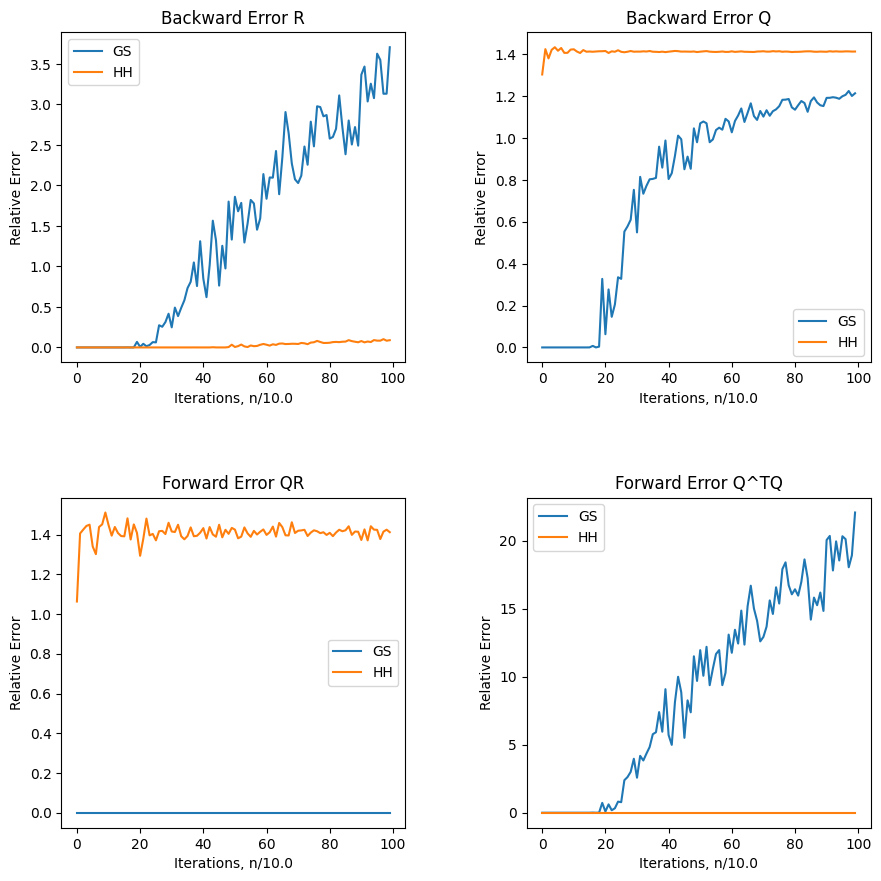
\includegraphics[width = 0.9\textwidth]{Images/problem6d MC3.png}
        \caption{Relative Errors for Gram Schmidt (GS) and Hausholder (HH) QR.}
        \label{fig:enter-label}
    \end{figure}

\clearpage
\begin{lstlisting}
import numpy as np
from IPython.display import display, clear_output
import matplotlib.pyplot as plt
def calculate_Hausholder(v: np.array):
    """
    Helper function to calculate the Hausholder matrix from v.
    
    Parameters
    ----------
    v : np.array
        The given vector. Needs to be normalized prior to passing.
        
    Returns
    -------
    H : np.ndarray
        The Hausholder matrix of v.
    """
    
    H = np.identity(max(v.shape)) - 2*np.outer(v, v)
    return H


def my_qr(A: np.ndarray):
        """
        Returns the QR factorization of a nonsingular array
        via (classical) Gram-Schmidt.

        Parameters
        ----------
        A: np.ndarray
            The matrix with which we find the QR factorization.
            Must be nonsingular, sized n x n

        Returns
        -------
        Q: np.ndarray
            A set of orthonormal column vectors of size n x n

        R: np.ndarray
            An upper triangular matrix
        """
        m, n = A.shape
        Q = np.zeros((m, m))
        R = np.zeros((m, n))

        for i in range(0, m): #Row Iter
            prev = 0 # used to catch r_{jk}q_j in sum
            for j in range(0, i+1): # maintain upper triangularity
                if i != j:
                    R[j, i] = np.dot(Q[:, j], A[:, i])
                    prev += R[j, i] * Q[:, j]
                else: #Diagonal term, take prev
                    R[i, i] = np.linalg.norm(A[:, i] - prev, ord = 2)
                    assert R[i, i] != 0, "Diagonal is zero, function cannot continue"
                    Q[:, j] = (1/R[i, i]) * (A[:, i] - prev)
    
        return Q, R
    
def hausholder_qr(A: np.ndarray):
    """
        Returns the QR factorization obtained through 
        the Hausholder Reflection method. 
        
        Elements belonging to and above diagonal are R, 
        
        Below the diagonal are the column vectors v_1, ..., v_n-1
        which are used to get Q_1, ..., Q_n-1. 
        
        Last element of v_i is not stored. Can be recovered since 
        v is a unit vector.
    """
    m, n = A.shape
    v_mat = []
    for i in range(m-1):
        
        # Obtaining v_i
        u = A[i:, i].copy()
        u[0] -= np.linalg.norm(u, ord = 2)
        v = u/np.linalg.norm(u, ord = 2)
        
        v_mat.append(v)

        #Calculating Q only to get next iteration
        Q = np.identity(m)
        Q[i:, i:] = calculate_Hausholder(v)
        
        A = np.matmul(Q, A)

    #Storing v_i's
    for i in range(m-1):
        A[i+1:, i] = np.array(v_mat[i])[:-1]
        
    return A

def recover_Qis(A: np.ndarray):
    """
    Calculates all Q_is from a Hausholder applied matrix A.
    
    Parameters
    ----------
    
    A : np.ndarray
        The matrix on which Hausholder QR has been performed
        
    Returns
    -------
    Qis : list(np.ndarray)
        A list containing all Q's 
    """
    Qis = []
    
    m, n = A.shape
    
    for i in range(m - 1):
        v = np.zeros(m - i)
        v[1:] = A[i+1:, i].copy()
        v[0] = np.sqrt(1 - np.linalg.norm(v, ord = 2)**2)
        Q = np.identity(m)
        Q[i:, i:] = calculate_Hausholder(v)
        Qis.append(Q)
    
    return Qis

def calculate_Q(A: np.ndarray):
    """
    Returns the orthonormal matrix Q from the matrix A after Hausholder QR 
    is applied.
    
    Parameters
    ----------
    
    A : np.ndarray
        The matrix on which Hausholder QR has been performed

    Returns
    -------    
    
    Q: np.ndarray
        The orthonormal matrix involved in QR
    """
    
    Qis = recover_Qis(A.copy())
    Q = np.identity(Qis[0].shape[0])
    for Qi in Qis:
        Q = np.matmul(Q, Qi.T)
        
    return Q

def Rel_error(A : np.ndarray, B : np.ndarray) -> float:
    """
    Helper function to calculate the relative error of two matrices.
    Relative error is taken with respect to A, and with the 
    Frobenius norm
    """
    
    num = np.linalg.norm(A - B, ord='fro')
    den = np.linalg.norm(A, ord = 'fro')
    return num * (1/den)
\end{lstlisting}
\begin{lstlisting}
maxsize = 1000
iterations = 100

i = 0

#Result array. 
#Size Quantity x iterations x number of functions
res = np.ndarray((4, iterations, 2))

for n in range(int(maxsize/iterations), maxsize +1 , int(maxsize/iterations)):
    
    
    #Temporary array to store quantities. 
    #Only holds one set of Quants at a time. 
    res_arr = np.zeros(4)
    
    #Get a random upper triangular matrix. Size will increase
    R = np.triu(np.random.default_rng().normal(10, 2.5, size=(n, n)))

    # Get a random matrix.
    B = np.random.default_rng().normal(10, 2.5, size=(n, n))
    Q = np.linalg.qr(B)[0]

    #Form A = QR
    A = np.matmul(Q, R)
    
    #Identity matrix
    I = np.identity(n)
    
    #QR from the Gram schmidt QR
    GS_Q, GS_R = my_qr(A)

    #Forward Errors for GS
    GS_A = np.matmul(GS_Q, GS_R)
    GS_I = np.matmul(GS_Q.T, GS_Q)
    
    #QR from HausHolder QR
    HH = hausholder_qr(A)
    HH_Q = calculate_Q(HH)
    HH_R = np.triu(HH)
    
    #Forward errors for HH
    HH_A = np.matmul(HH_Q, HH_R)
    HH_I = np.matmul(HH_Q.T, HH_Q)

    #Calcualting relative error for GS
    res_arr = np.array([Rel_error(R, GS_R), 
                        Rel_error(Q, GS_Q), 
                        Rel_error(A, GS_A), 
                        Rel_error(I, GS_I) 
                        ])
    
    #Storing GS results for iteration 
    res[:, i, 0] = res_arr
    
    #Calculating relative error for HH
    res_arr = np.array([Rel_error(R, HH_R),
                        Rel_error(Q, HH_Q),
                        Rel_error(A, HH_A),
                        Rel_error(I, HH_I)])
    
    #Storing HH results for iteration
    res[:, i, 1] = res_arr
    
    #Incrementing for next iteration
    i+=1
    
    #Clearing output
    clear_output(wait=True)
    
    print("Percentage done: {:.2f}%".format(100*n/maxsize))
\end{lstlisting}
\begin{lstlisting}
Titles = ["Backward Error R", "Backward Error Q", "Forward Error QR", "Forward Error Q^TQ"]
method = ["GS", "HH"]
fig, ax = plt.subplots(2, 2, figsize=(10, 10))
for i in range(2):
    for j in range(2):
        index = i * 2 + j
        ax[i, j].set_title(Titles[index])
        
        for k in range(2):
            ax[i, j].plot(res[index, :, k], label=method[k])
            ax[i, j].legend()
            
        ax[i, j].set_xlabel(f'Iterations, n/{maxsize / iterations}')
        ax[i, j].set_ylabel("Relative Error")

plt.tight_layout(pad=5.0)
plt.show()
\end{lstlisting}
\end{solution}

\subsection{Problem 6, part e}
Create a \textit{Vandermonde matrix} and a vector,
\[
A = \mqty[
    1 &\alpha_0 &\alpha_0^2 &\dots &\alpha_0^{n-1} \\
    1 &\alpha_1 &\alpha_1^2 &\dots &\alpha_1^{n-1} \\
    1 &\alpha_2 &\alpha_2^2 &\dots &\alpha_2^{n-1} \\
    \vdots &\vdots &\vdots &\ddots &\vdots\\
    1 &\alpha_{m - 1} &\alpha_{m - 1}^2 &\dots &\alpha_{m - 1}^{n-1} 
        ]
        \in \R^{m\times n}, 
        \hspace{5mm}
        \textbf{b} = 
        \mqty[
        \exp (\sin 4\alpha_0)\\
        \exp (\sin 4\alpha_1)\\
        \exp (\sin 4\alpha_2)\\
        \vdots \\
        \exp (\sin 4\alpha_{m - 1})
        ] \in \R^m,
\]
where $\alpha_i = i/(m-1), i = 0, ..., m-1$. This arises when we try to do polynomial fitting
\[
e^{\sin(4x)} \approx c_0 + c_1x + x_2x^2 + \dots + c_{n-1}x^{n-1}
\]
over the interval $[0, 1]$ at discrete points $x = 0, \frac{1}{m-1}, \dots, \frac{m - 2}{m - 1}, 1$. For $n = 15$ and $m = 100$, solve the least squares problem $\min \norm{A\textbf{x} - \textbf{b}}_2$ and state your value of $c_{14}$ using each of the following methods.
\begin{enumerate}[(i)]
    \item Applying $QR$ Factorization to $A$.
    \item Applying $QR$ Factorization to the augmented matrix $[A, \textbf{b}] \in \R^{m \times (n+1)}$.
    \item Solving the normal equations $A^TA\textbf{x} = A^T\textbf{b}.$
\end{enumerate}
For (i) and (ii), your code should show how the respective $QR$ factors are used in obtaining a solution of the least squares problem. Your are free to use your program's built-in functions for solving linear systems but for other things, use that you have implemented in (a), (b), (c). The true value of $c_{14}$ is 2006.787453080206....Comment on the accuracy of each method and algorithm.
\end{document}